\appendix
\chapter{First Appendix}
\section{Feature description}
The information in this table is from the Spotify Web API website \cite{SpotifyFeatures:online}.

\begin{longtable}{|p{3cm}|p{1.6cm}|p{7cm}|}
% \begin{tabular}{|p{3cm}|p{2cm}|p{7cm}|}
\hline
\textbf{Feature name}     & \textbf{Feature type} & \textbf{Feature description}                                                                                                                                                                                                                                                                                                                                                                                                                                                                                                \\ \hline \hline
\endhead
duration\_ms     & int          & The duration of the track in milliseconds.                                                                                                                                                                                                                                                                                                                                                                                                                                                                         \\ \hline
key              & int          & The estimated overall key of the track. Integers map to pitches using standard Pitch Class notation . E.g. 0 = C, 1 = C♯/D♭, 2 = D, and so on. If no key was detected, the value is -1.                                                                                                                                                                                                                                                                                                                            \\ \hline
mode             & int          & Mode indicates the modality (major or minor) of a track, the type of scale from which its melodic content is derived. Major is represented by 1 and minor is 0.                                                                                                                                                                                                                                                                                                                                                    \\ \hline
time\_signature  & int          & An estimated overall time signature of a track. The time signature (meter) is a notational convention to specify how many beats are in each bar (or measure).                                                                                                                                                                                                                                                                                                                                                      \\ \hline
acousticness     & float        & A confidence measure from 0.0 to 1.0 of whether the track is acoustic. 1.0 represents high confidence the track is acoustic.                                                                                                                                                                                                                                                                                                                                                                                       \\ \hline
danceability     & float        & Danceability describes how suitable a track is for dancing based on a combination of musical elements including tempo, rhythm stability, beat strength, and overall regularity. A value of 0.0 is least danceable and 1.0 is most danceable.                                                                                                                                                                                                                                                                       \\ \hline
energy           & float        & Energy is a measure from 0.0 to 1.0 and represents a perceptual measure of intensity and activity. Typically, energetic tracks feel fast, loud, and noisy. For example, death metal has high energy, while a Bach prelude scores low on the scale. Perceptual features contributing to this attribute include dynamic range, perceived loudness, timbre, onset rate, and general entropy.                                                                                                                          \\ \hline
instrumentalness & float        & Predicts whether a track contains no vocals. “Ooh” and “aah” sounds are treated as instrumental in this context. Rap or spoken word tracks are clearly “vocal”. The closer the instrumentalness value is to 1.0, the greater likelihood the track contains no vocal content. Values above 0.5 are intended to represent instrumental tracks, but confidence is higher as the value approaches 1.0.                                                                                                                 \\ \hline
liveness         & float        & Detects the presence of an audience in the recording. Higher liveness values represent an increased probability that the track was performed live. A value above 0.8 provides strong likelihood that the track is live.                                                                                                                                                                                                                                                                                            \\ \hline
loudness         & float        & The overall loudness of a track in decibels (dB). Loudness values are averaged across the entire track and are useful for comparing relative loudness of tracks. Loudness is the quality of a sound that is the primary psychological correlate of physical strength (amplitude). Values typical range between -60 and 0 db.                                                                                                                                                                                       \\ \hline
speechiness      & float        & Speechiness detects the presence of spoken words in a track. The more exclusively speech-like the recording (e.g. talk show, audio book, poetry), the closer to 1.0 the attribute value. Values above 0.66 describe tracks that are probably made entirely of spoken words. Values between 0.33 and 0.66 describe tracks that may contain both music and speech, either in sections or layered, including such cases as rap music. Values below 0.33 most likely represent music and other non-speech-like tracks. \\ \hline
valence          & float        & A measure from 0.0 to 1.0 describing the musical positiveness conveyed by a track. Tracks with high valence sound more positive (e.g. happy, cheerful, euphoric), while tracks with low valence sound more negative (e.g. sad, depressed, angry).                                                                                                                                                                                                                                                                  \\ \hline
tempo            & float        & The overall estimated tempo of a track in beats per minute (BPM). In musical terminology, tempo is the speed or pace of a given piece and derives directly from the average beat duration. \\ \hline
% \end{tabular}
\caption{Table containing feature description}
\label{tab:feature}
\end{longtable}

% Fix to move content to next page
\vspace{300pt}

\section{Additional figues}
\begin{figure}[h]
\centering
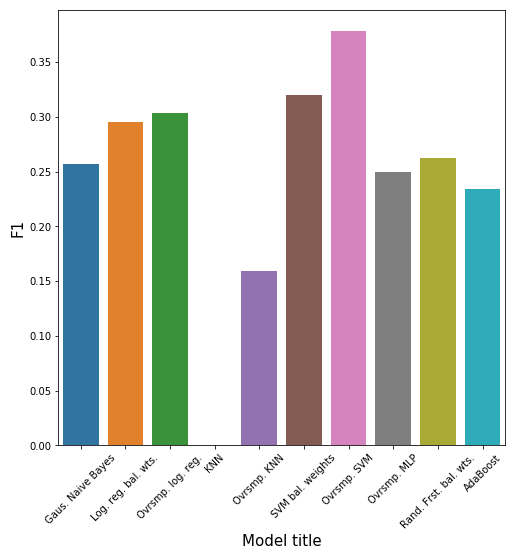
\includegraphics[width=0.62\linewidth]{appendix/fig/f1s.PNG}
\caption{Model F1 scores}
\label{fig:f1s}
\end{figure}
% \vspace{-700pt}
\begin{figure}[h]
\centering
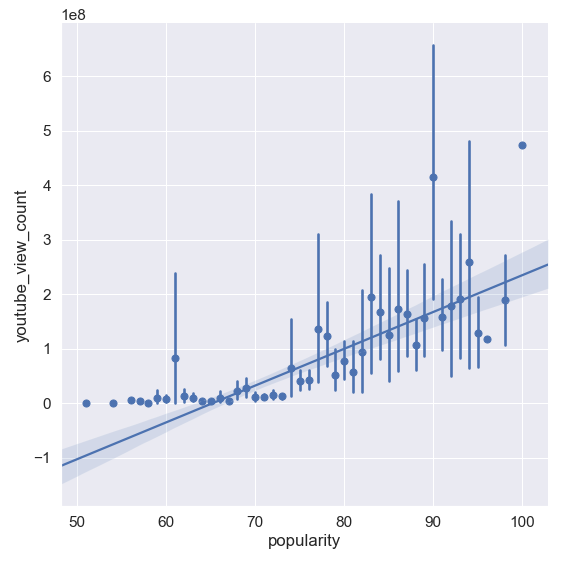
\includegraphics[width=0.62\linewidth]{appendix/fig/correlation.PNG}
\caption{Youtube view count and popularity correlation}
\label{fig:ytcor}
\end{figure}

% \section{Full scores table}

% This is a table presenting all the different evaluation metrics used for every model. It looks at Accuracy, Specificity, Recall, Precision, F1 score, AUC and Generalisation AUC.

% On top of Accuracy, Specificity, Recall, Precision, F1 score and AUC this table also includes Average Precision (AP). It is meant to summarise the precision-recall curve (a curve similar to the ROC curve but it plots Precision and Recall for every threshold instead of Recall and False Positive Rate). It is supposed to be a good indication of model performance in imbalanced data sets. A more in-depth description is found in the sci-kit learn documentation \cite{sklearnAP:online}.

% \begin{table}
% % \begin{adjustbox}{max width=\textwidth}
% \resizebox{\textwidth}{!}{%
% \begin{tabular}{*{8}{|c}|}
% \hline
% \textbf{Model title}    & \textbf{Acc.} & \textbf{Spec.} & \textbf{Rec.} & \textbf{Prec.} & \textbf{F1} & \textbf{AUC} & \textbf{Gen. AUC}\\ \hline
% Gaussian Naive Bayes    & 0.404             & 0.339                & 0.940                        & 0.149              & 0.257       & 0.670        & 0.421                           \\ \hline
% Log. reg. bal. weights. & 0.639             & 0.634                & 0.680                        & 0.191              & 0.296       & 0.745        & 0.433                          \\ \hline
% Over-sampling log. reg.  & 0.641             & 0.632                & 0.720                        & 0.194              & 0.304       & 0.730        & 0.454                           \\ \hline
% KNN                     & 0.891             & 1.000                & 0.000                        & 0.000              & 0.000       & 0.560        & 0.685                           \\ \hline
% Over-sampling KNN        & 0.739             & 0.802                & 0.220                        & 0.130              & 0.159       & 0.511        & 0.478                           \\ \hline
% SVM bal. weights        & 0.628             & 0.607                & 0.800                        & 0.203              & 0.320       & {\ul 0.772}  & 0.566                          \\ \hline
% Over-sampling SVM        & 0.743             & 0.749                & 0.700                        & 0.270              & {\ul 0.378} & 0.770        & 0.481                          \\ \hline
% Over-sampling MLP        & 0.843             & 0.915                & 0.260                        & 0.248              & 0.250       & 0.693        & 0.572                          \\ \hline
% Random Forest bal. wts. & 0.733             & 0.768                & 0.440                        & 0.190              & 0.262       & 0.676        & 0.382                           \\ \hline
% AdaBoost                & 0.843             & 0.917                & 0.240                        & 0.235              & 0.234       & 0.633        & 0.486                           \\ \hline
% \end{tabular}%
% }
% \caption{Table containing model scores}
% \label{tab:modelscores}
% \end{table}

% \begin{longtable}{|p{2.5cm}|p{1cm}|p{1cm}|p{1cm}|p{1cm}|p{1cm}|p{1cm}|p{1cm}|p{1cm}|}
% \hline
% \textbf{Model title}    & \textbf{Acc.} & \textbf{Spec.} & \textbf{Rec.} & \textbf{Prec.} & \textbf{F1} & \textbf{AUC} & \textbf{Gen. AUC}\\ \hline
% Gaussian Naive Bayes    & 0.404             & 0.339                & 0.940                        & 0.149              & 0.257       & 0.670        & 0.421                           \\ \hline
% Log. reg. bal. weights. & 0.639             & 0.634                & 0.680                        & 0.191              & 0.296       & 0.745        & 0.433                          \\ \hline
% Over-sampling log. reg.  & 0.641             & 0.632                & 0.720                        & 0.194              & 0.304       & 0.730        & 0.454                           \\ \hline
% KNN                     & 0.891             & 1.000                & 0.000                        & 0.000              & 0.000       & 0.560        & 0.685                           \\ \hline
% Over-sampling KNN        & 0.739             & 0.802                & 0.220                        & 0.130              & 0.159       & 0.511        & 0.478                           \\ \hline
% SVM bal. weights        & 0.628             & 0.607                & 0.800                        & 0.203              & 0.320       & {\ul 0.772}  & 0.566                          \\ \hline
% Over-sampling SVM        & 0.743             & 0.749                & 0.700                        & 0.270              & {\ul 0.378} & 0.770        & 0.481                          \\ \hline
% Over-sampling MLP        & 0.843             & 0.915                & 0.260                        & 0.248              & 0.250       & 0.693        & 0.572                          \\ \hline
% Random Forest bal. wts. & 0.733             & 0.768                & 0.440                        & 0.190              & 0.262       & 0.676        & 0.382                           \\ \hline
% AdaBoost                & 0.843             & 0.917                & 0.240                        & 0.235              & 0.234       & 0.633        & 0.486                           \\ \hline
% \caption{Table containing model scores}
% \label{tab:modelscores}
% \end{longtable}
